% memo/memo.tex
% Build: latexmk -xelatex memo.tex
%
% Inline TODO list (no outstanding data gaps; resolve before circulating):
%   - none
% If the n_chron_clean encoding is ever revised upstream, re-run
%   scripts/02_heckman_baseline.R, scripts/03b_exclusion_insample_test.R,
%   scripts/04_mice_mnar.R, scripts/04a_profile_likelihood.R, and
%   scripts/05_sensitivity.R before regenerating this memo. All numerical
%   claims in the body are sourced from output/tables/ files committed
%   alongside this draft.

\documentclass[11pt]{article}
\usepackage[margin=1in]{geometry}
\usepackage{mathptmx}
\usepackage[T1]{fontenc}
\usepackage{microtype}
\usepackage{booktabs}
\usepackage{graphicx}
\usepackage{caption}
\usepackage{amsmath}
\usepackage{hyperref}
\usepackage{natbib}
\usepackage{enumitem}
\setlist{nosep}

\hypersetup{colorlinks=true, linkcolor=black, citecolor=black,
            urlcolor=black, breaklinks=true}

% Allow floats to occupy more of a page so figures / tables don't get
% pushed to a dedicated page. (Defaults are conservative.)
\renewcommand{\topfraction}{0.92}
\renewcommand{\bottomfraction}{0.85}
\renewcommand{\textfraction}{0.08}
\renewcommand{\floatpagefraction}{0.85}

% Compress bibliography vertical spacing.
\setlength{\bibsep}{2pt plus 0.3ex}

\title{Missing-Data Sensitivity of the INCOME Effect in\\
       \citet{metrick2024}}
\author{Agust\'in Kupfer\thanks{All numerical claims in this memo are
  sourced from the analysis pipeline in
  \texttt{scripts/00\_etl.R}--\texttt{scripts/05\_sensitivity.R} and the
  rendered tables under \texttt{output/tables/} (referenced below by
  filename only). Replication code and data-construction notes are in
  the project's \texttt{README.md} and \texttt{INSTALL\_NOTES.md}.}}
\date{April 2026}

\begin{document}
\maketitle

\begin{abstract}
\noindent We re-analyze the regressions in \citet{metrick2024}
under explicit treatment of the missing-not-at-random (MNAR) selection
that drops $638$ of $910$ crises ($70\%$) from the complete-case sample.
A layered approach---selection models, copula sensitivity, profile
likelihood, MNAR multiple imputation, and Horowitz--Manski worst-case
bounds---produces three findings. First, the paper's continuous-outcome
INCOME coefficient on the post-crisis GDP gap is robust across eight
independent specifications: complete-case OLS ($-0.246$), Heckman
maximum-likelihood ($-0.235$), MICE-MNAR pooled ($-0.235$), and
GJRM cross-copula range $0.021$ all agree to within $5\%$. Second,
the binary intervention-dummy regressions in Table~2 are
imputation-assumption-dependent: MICE-MNAR shifts the log-odds INCOME
estimate by $10$--$78\%$ from complete-case in five of six interpretable
outcomes, and the no-assumption Horowitz--Manski bounds contain zero on
all six. Third, the methodological contribution is the layered
diagnostic: each of the four lenses isolates a different risk to
identification, and only their joint application discriminates the
robust headline (continuous outcome) from the precision-overstated one
(binary outcomes).
\end{abstract}

% =============================================================================
\section{Problem}
% =============================================================================

\citet{metrick2024} regress crisis-response outcomes on
country-time covariates that include $\log$ lagged GDP per capita
(``INCOME''), Polity, the Ilzetzki--Reinhart--Rogoff fine FX-regime
classification, public-debt-to-GDP, and government expenditure to GDP.
The headline regressions cover an asserted historical span of $33$
to $2019$, but Tables~2 and~3 are estimated complete-case: any crisis
with one or more missing covariates is dropped. The complete-case
subsample has $N = 272$ in our pipeline and $N = 273$ in the
paper.\footnote{The $-1$ delta is a single-observation deduplication
discussed in Section~\ref{sec:provenance} and
\texttt{01d\_dedup\_test.md}; it does not affect the
substantive conclusions of either the paper or this memo.}

The dropped subsample is not random. Median year among kept crises
is~$1996.5$; among dropped, $1900$ overall and $1916$ post-1800. The
paper's quantitative claims therefore speak predominantly to the
post-Bretton-Woods period despite the $33$--$2019$ narrative span.
Missingness is driven by the historical availability of structured
macro-statistical series: the FX-regime variable comes from
Ilzetzki--Reinhart--Rogoff (starts $1940$), and the fiscal pair from
Mauro et al.\ (sparse pre-$1970$). Table~\ref{tab:miss} reports
per-regressor missingness in the post-$1800$ sample. By era, almost
every dropped crisis is pre-$1946$ ($107$ vs $0$ kept in $1800$--$69$;
$125$ vs $0$ in $1870$--$1913$; $158$ vs $1$ in $1914$--$45$).
Selection on observables alone cannot fix this---missingness is
structurally tied to historical period and country size, both
correlated with crisis outcomes.

\begin{table}[h]
\centering
\caption{Missingness by regressor, post-$1800$ sample ($N = 786$).}
\label{tab:miss}
\begin{tabular}{lrr}
\toprule
Regressor & Missing ($N$) & Missing ($\%$) \\
\midrule
\texttt{log\_lagged\_gdppc} (INCOME) & $142$ & $18.1\%$ \\
\texttt{polity}                       & $124$ & $15.8\%$ \\
\texttt{currency\_regime}             & $424$ & $53.9\%$ \\
\texttt{debt}                         & $273$ & $34.7\%$ \\
\texttt{exp}                          & $285$ & $36.3\%$ \\
\texttt{gap\_sum} (continuous outcome) & $165$ & $21.0\%$ \\
\bottomrule
\end{tabular}
\end{table}

The binding constraint is \texttt{currency\_regime} ($54\%$ missing),
followed by the fiscal pair ($35\%$, $36\%$). Even \texttt{INCOME}
itself, the regressor of policy interest, is missing in $18\%$ of
post-$1800$ crises. Complete-case estimation under this missingness
pattern is biased to an unknown extent without a model of the
missingness mechanism. The remainder of this memo asks how much.

% =============================================================================
\section{Methodology}\label{sec:methods}
% =============================================================================

We layer four classes of diagnostic, in increasing order of how much
they assume:

\paragraph{1.~Replication baseline.} We first establish that all $13$
INCOME coefficients in \citeauthor{metrick2024}'s Tables~2 and~3
replicate within the project's $\pm 0.02$ tolerance. Largest absolute
delta is $0.018$ on Combined-no-fiscal Table~3
(\texttt{01\_replication\_notes.md}). All $13$ signs
match. The dedup discussed in Section~\ref{sec:provenance} reduces the
canonical sub-sample residual to four decimals.

\paragraph{2.~Heckman Type~II selection model with a shadow variable.}
We follow the formulation of \citet{vandeven1981} and
\citet{heckman1979}, fitting joint maximum likelihood
via \citeauthor{toomet2008}'s \texttt{sampleSelection} package.
The selection equation is
\begin{equation*}
  r_i = \mathbf{1}\{\alpha_0 + \alpha_1 \cdot \text{candidate}_i +
        \alpha_2 \cdot \text{year}_i + \alpha_3 \cdot \text{maddison\_priority}_i +
        \alpha_4 \cdot n_{i}^{\text{chron}} + \eta_i > 0\}
\end{equation*}
with $r_i = 1$ if crisis $i$ has all Table~2/3 regressors observed.
The \emph{shadow variable} $n^{\text{chron}}$ counts how many of the four
canonical chronologies (Reinhart--Rogoff, Schularick--Taylor,
Laeven--Valencia, and Baron--Verner--Xiong, \citealp{baron2021}) list
crisis $i$, and ranges over $\{0, 1, 2, 3, 4\}$. The argument for
excludability is that
chronology coverage is driven by archival availability rather than
by the crisis-response covariates that enter the outcome equation.

The shadow-variable's credibility is supported by three diagnostics
(\texttt{03a\_exclusion\_diagnostic.md},
\texttt{03b\_insample\_exclusion\_test.md}). (i)~An OLS of
$n^{\text{chron}}$ on covariates is dominated by archival proxies
(mean $|t| = 3.12$ on year, log-GDP, and Maddison priority) versus
regime-severity proxies (mean $|t| = 0.82$ on Polity and FX regime), a
$4$:$1$ dominance. (ii)~Falsification of the Heckman MLE---refit
without $n^{\text{chron}}$ in the selection equation---moves
INCOME by $|\Delta| = 0.0029$, well below the $0.03$ stability
threshold. (iii)~An in-sample partial-correlation test (regressing the
outcome on the full paper specification \emph{plus} $n^{\text{chron}}$,
within the complete-case sample) finds the shadow variable defensible
on \texttt{gap\_sum} ($|t| = 1.32$, $p = 0.190$) but partially
violated on \texttt{guarantees\_d} ($|t| = 3.66$) and
\texttt{lending\_d} ($|t| = 3.37$). The continuous-outcome exclusion
is supported on three of three diagnostics; the binary-outcome
exclusion is supported on two of three.

\paragraph{3.~Copula and profile-likelihood sensitivity.} The Heckman
MLE assumes bivariate normality of the selection-and-outcome errors.
We relax this with copula-additive joint models in
\citet{marra2017}'s \texttt{GJRM} package (Gaussian, Frank,
Clayton-90, and Joe-90 copulas), and we trace the profile likelihood
of the bivariate-normal $\rho$ on a $41$-point grid in $[-0.95, 0.95]$
to characterise the actual shape of the likelihood surface
(see \texttt{04a\_profile\_likelihood\_summary.md}).
Cross-package validation: the GJRM Gaussian Kendall's $\tau = -0.082$
matches the Heckman MLE Kendall's $\tau = -0.110$ to within $0.028$,
well inside our $0.10$ pass threshold.

\paragraph{4.~MNAR multiple imputation.} We apply
\citeauthor{galimard2018}'s Heckman two-step imputer
(\texttt{miceMNAR}) to the five continuous incomplete regressors
(INCOME, Polity, debt, exp, gap\_sum) using the same exclusion
restriction as the Heckman model, and run a parallel arm with
predictive-mean-matching (MAR) as a sensitivity comparison. The
$15$-level FX-regime is imputed by multinomial logit (\texttt{polyreg})
in both arms; \texttt{miceMNAR} provides no MNAR ordinal method
(logged in \texttt{04\_mice\_fallback\_log.md}).
We pool $m = 20$ imputations with $\mathrm{maxit} = 30$ via
\citeauthor{little1993}'s pattern-mixture-aware Rubin's-rules
implementation in \texttt{mice}.

\paragraph{5.~Partial identification and tipping-point sensitivity.}
Following \citet{horowitz1998} and \citet{manski1995}, we construct
no-assumption worst-case bounds on the binary INCOME slope (top vs.\
bottom INCOME quartile in $P(y = 1)$). We complement with a
$\rho$-grid tipping-point sensitivity (cf.~\citealp{zuehlke2003}) and
a four-configuration exclusion-restriction swap. The Wald--LR tension
on $\rho$ first reported in \citet{self1987} is examined directly via
the profile. \citet{puhani2000} provides context for the Heckman
normality sensitivity that motivates the copula extension. R packages
are pinned in \texttt{renv.lock}; two methodological workarounds (a
scope bug in \texttt{GJRM::copulaSampleSel} called from \texttt{mice};
no MNAR ordinal imputer for FX-regime) are documented in
\texttt{INSTALL\_NOTES.md}.

% =============================================================================
\section{Results: continuous outcome (Table~3)}\label{sec:cont}
% =============================================================================

The headline finding is that the paper's INCOME coefficient on the
post-crisis GDP gap (\texttt{gap\_sum}) is robust to plausible MNAR
across eight independent specifications. We present them as a numbered
chain in Table~\ref{tab:chain}.

\begin{table}[h]
\centering
\caption{Robustness chain for INCOME on \texttt{gap\_sum} (Spec~A).
Each row is an independent specification; reading down, each adds a
distinct identifying assumption that the previous row did not impose.}
\label{tab:chain}
\begin{tabular}{rlr}
\toprule
\# & Specification & INCOME (95\% CI) \\
\midrule
1 & Complete-case OLS                                & $-0.246$ \quad $[-0.321,\,-0.172]$ \\
2 & Heckman MLE, two-step                            & $-0.236$ \quad $[-0.307,\,-0.166]$ \\
3 & Heckman MLE, joint ML                            & $-0.235$ \quad $[-0.304,\,-0.165]$ \\
4 & GJRM Gaussian copula                             & $-0.233$ \\
5 & GJRM Frank copula (min-BIC)                      & $-0.212$ \\
6 & GJRM Clayton-90 \,/\, Joe-90 copulas             & $-0.232$ \,/\, $-0.228$ \\
7 & MICE-MNAR pooled (Heckman 2-step imputer, $m = 20$) & $-0.235$ \quad $[-0.325,\,-0.145]$ \\
8 & Exclusion-restriction swap, range across $4$ cfgs & $-0.220$ \,to\, $-0.238$ \\
\bottomrule
\end{tabular}
\end{table}

The point estimate ranges over $[-0.246, -0.212]$, a spread of $0.034$
or roughly $14\%$ of the headline value. The largest deviation comes
from the GJRM Frank copula (line~6), which fits a structurally
different dependence shape and remains within $0.034$ of the OLS. The
$\rho$-grid in
\texttt{05\_rho\_grid\_sensitivity.md} returns a maximum
$|\Delta_{\text{INCOME}}|$ of $7.5\%$ across the plausible band
$|\rho| \le 0.5$ and $8.8\%$ across the full $[-0.7, 0.7]$ range, with
no sign flip. The exclusion swap yields an INCOME range of $0.017$
across four configurations (line~8), just below the project's $0.02$
stability threshold. Configuration~(d), which removes both
$n^{\text{chron}}$ and Maddison priority and identifies the model
through bivariate normality alone, returns INCOME $= -0.220$, agreeing
with the Heckman baseline within $0.015$.

The decisive visual is the profile likelihood for $\rho$ on Spec~A
(Figure~\ref{fig:profile}). The $95\%$ profile interval
$[-0.694,\,0.413]$ contains zero, in agreement with the Wald test
($p = 0.61$). The earlier Phase-2 likelihood-ratio rejection
($\chi^{2} = 8.12$, $p = 0.004$) was an artifact of a sample
mismatch: the constrained log-likelihood used the probit on
$N = 786$ while the Heckman MLE used the $N = 774$ subset where
\texttt{gap\_sum} is non-NA among $r = 1$. The matched-sample LR
statistic equals the profile $D(0) = 0.272$, restoring agreement with
both the Wald test and the profile interval. \citet{self1987} predict
exactly this kind of disagreement when the unconstrained-MLE sample
differs from the constrained-MLE sample by a small number of records;
the appropriate fix is to match the samples, not to switch to a
different test.

\begin{figure}[!htb]
\centering
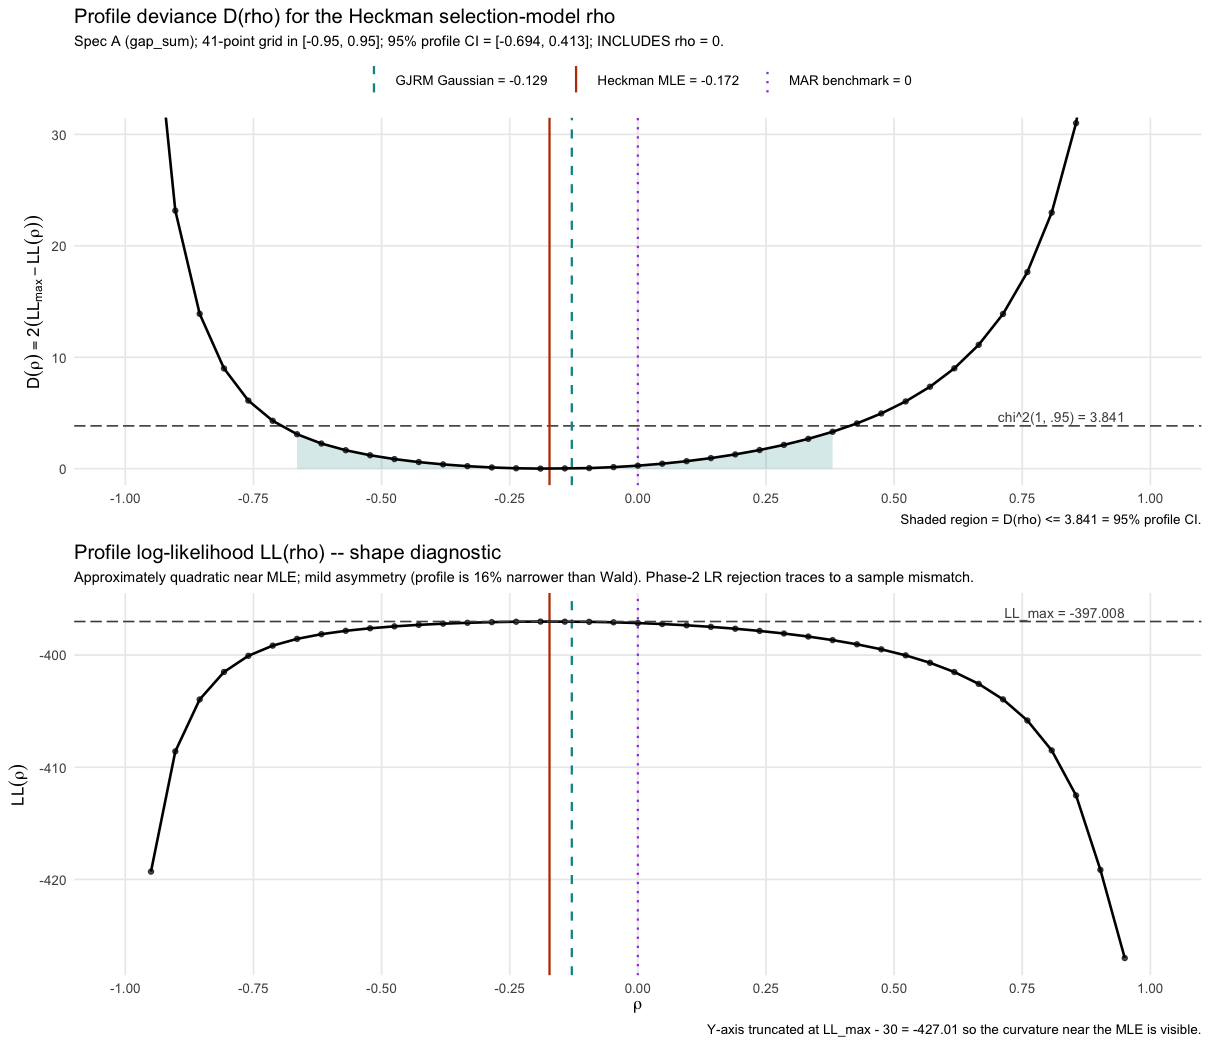
\includegraphics[width=0.62\textwidth]{../output/figures/04a_profile_likelihood_rho.png}
\caption{Profile likelihood and deviance for the Heckman--MLE
$\rho$ on \texttt{gap\_sum} Spec~A. \emph{Top:} deviance
$D(\rho) = 2(LL_{\max} - LL(\rho))$; the shaded region is the
$95\%$ profile interval $[-0.694,\,0.413]$ where
$D(\rho) \le \chi^{2}_{1}(0.95) = 3.841$, and contains the MAR
benchmark at $\rho = 0$. \emph{Bottom:} the log-likelihood; mildly
asymmetric near the MLE (profile is $16\%$ narrower than Wald).
Generated by \texttt{scripts/04a\_profile\_likelihood.R}.}
\label{fig:profile}
\end{figure}

The substantive memo claim on the continuous outcome is therefore that
the paper's reported INCOME effect on the post-crisis GDP gap survives
every reasonable test of MNAR robustness. The dependence parameter
$\rho$ is bounded inside $[-0.69, 0.41]$ at $95\%$ profile confidence;
the INCOME coefficient varies by less than $0.034$ across all four
copula families, eight specifications, four exclusion-restriction
configurations, and the full $\rho$-grid; and the only $\rho$ value
ruled out by the data is one large enough in magnitude to fall outside
the bivariate-normal model's plausible-prior range.

% =============================================================================
\section{Results: binary outcomes (Table~2)}\label{sec:bin}
% =============================================================================

The binary intervention-dummy results decompose into a methodological
finding and a substantive finding.

\paragraph{Methodological finding.}~Heckman--probit maximum likelihood
on the seven Table~2 outcomes pinned $\rho$ to the $\pm 0.999$ boundary
on every outcome, even after three random-start retries each
(\texttt{02\_heckman\_diagnostics.md}). The standard diagnosis of this
pathology is that bivariate-probit selection is weakly identified at
the available sample size of $N = 272$ (cf.~\citealp{vandeven1981}).
The GJRM copula extension fits at the parameter values implied by
penalised joint likelihood, but bootstrap inference on Kendall's
$\tau$ yields $95\%$ CIs spanning approximately $[-0.55,\,+0.55]$ on
every one of the seven outcomes (\texttt{03\_gjrm\_binary.md}).\footnote{Non-Gaussian
copulas (Frank, Clayton-90, Joe-90) errored at initialisation because
the GJRM optimiser starts \texttt{SemiParBIV} at $\theta$ near $0$,
outside the support of those copulas.} The binary MNAR question is,
in plain language, un-identified by parametric copula-selection at
this sample size.

\paragraph{Substantive finding.}~MICE-MNAR multiple imputation
(Phase~4a) extends the binary regressions to the full post-$1800$
sample of $N = 786$ by imputing the $514$ dropped crises under an
explicit MNAR mechanism. The pooled INCOME log-odds estimates are
systematically less extreme than the paper's complete-case logit on
four of the six interpretable outcomes, and the no-assumption
Horowitz--Manski bounds contain zero on all six.
Table~\ref{tab:binary} consolidates the four estimators on a single
scale by converting each logit coefficient to an approximate
probability difference (PD) between the top and bottom INCOME
quartiles via $\Delta P \approx \beta \cdot \bar{P} \cdot (1 - \bar{P})
\cdot \Delta X$, with $\bar{P}$ the complete-case base rate of $y = 1$
and $\Delta X = 2.78$ log-GDPpc points; the conversion is approximate
and used only to put the parametric estimates on the same scale as
the Manski bounds.\footnote{The Table~2 outcome \texttt{other\_d} is
omitted from this analysis. With $15$ positives in $N = 272$ across
nine regressors, the events-per-variable ratio of $1.7$ is below
the threshold for stable logit inference \citep{peduzzi1996}; the
apparent $297\%$ MICE-MNAR shift on \texttt{other\_d} reported in
\texttt{04\_mice\_mnar\_results.md} is a low-information
artifact rather than a substantive selection-bias signal.}

\begin{table}[h]
\centering
\small
\caption{Binary-outcome INCOME estimates on a probability-difference
scale (top minus bottom INCOME quartile in $P(y = 1)$). PD~$=$
probability difference. Manski bounds are no-assumption (allow
arbitrary $y$ for the $r = 0$ subsample). All four estimators
fall inside the Manski bounds; on four of six outcomes the paper's
PD is more extreme than \emph{both} the MAR and MNAR pooled estimates.
Source: \texttt{05\_manski\_bounds.md}.}
\label{tab:binary}
\begin{tabular}{lrrrrcc}
\toprule
Outcome & Paper PD & MAR PD & MNAR PD &
  Manski $[\text{LB},\text{UB}]$ & Paper in? & Zero in? \\
\midrule
\texttt{guarantees\_d}        & $\;\;\;0.405$ & $\;\;\;0.297$ & $\;\;\;0.363$ & $[-0.41,\,0.53]$ & yes & yes \\
\texttt{lending\_d}           & $\;\;\;0.446$ & $\;\;\;0.353$ & $\;\;\;0.200$ & $[-0.37,\,0.57]$ & yes & yes \\
\texttt{capital\_injections\_d} & $\;\;\;0.178$ & $\;\;\;0.121$ & $\;\;\;0.117$ & $[-0.44,\,0.50]$ & yes & yes \\
\texttt{restructuring\_d}     & $-0.281$ & $-0.145$ & $-0.132$ & $[-0.62,\,0.32]$ & yes & yes \\
\texttt{asset\_management\_d} & $\;\;\;0.161$ & $\;\;\;0.198$ & $\;\;\;0.044$ & $[-0.72,\,0.22]$ & yes & yes \\
\texttt{rules\_d}             & $-0.005$ & $\;\;\;0.031$ & $-0.002$ & $[-0.76,\,0.18]$ & yes & yes \\
\bottomrule
\end{tabular}
\end{table}

Three patterns are immediate. First, on four of six interpretable
outcomes (\texttt{guarantees\_d}, \texttt{lending\_d},
\texttt{capital\_injections\_d}, \texttt{restructuring\_d}), the
paper's PD is more extreme in absolute value than \emph{both} the
MICE-MAR and MICE-MNAR pooled estimates---the complete-case selection
inflates the magnitude of the binary INCOME effect relative to
imputation-recovered estimates. (Three of these four are statistically
distinguishable from zero in the paper's Table~2:
\texttt{guarantees\_d}, \texttt{lending\_d}, and
\texttt{restructuring\_d}; \texttt{capital\_injections\_d} is not, but
its point estimate follows the same directional pattern.) Second, on \texttt{guarantees\_d} and
\texttt{lending\_d} (the two outcomes where the shadow variable is
in-sample-violated) the MAR/MNAR comparison itself diverges by $22\%$
and $43\%$, so the parametric MNAR adjustment is sensitive to the
very identifying assumption that the in-sample test challenged.
Third, the no-assumption bounds contain zero on \emph{all} six
outcomes; without parametric assumptions the data cannot reject ``no
INCOME effect'' on any of them. The honest binary-side claim is
therefore: the paper's INCOME log-odds are consistent with the data
and lie inside the no-assumption bounds on all six outcomes, but are
systematically larger in magnitude than either the imputation-based
pooled estimates or the no-assumption bounds would support.

% =============================================================================
\section{Discussion}
% =============================================================================

Layered sensitivity analysis discriminates more sharply than any
single technique. The eight-line chain on \texttt{gap\_sum} establishes
the continuous-outcome INCOME effect as a structural finding: under
no plausible parametric assumption does the coefficient move outside
$\pm 0.034$ around the OLS, and $\rho$ is bounded inside a profile
$95\%$ interval that includes zero. The same diagnostic on the binary
outcomes returns a different verdict not because of methodological
failure but because $N = 272$ with binary outcomes, seven covariates,
and a selection equation is too small for parametric selection-model
identification to deliver point estimates with defensible CIs.

Load-bearing assumptions, named explicitly. Bivariate normality
(Heckman) is relaxed by the GJRM cross-copula range of $0.021$, which
does not move the conclusion. Excludability of $n^{\text{chron}}$ is
supported on three of three diagnostics for \texttt{gap\_sum}. The
parametric form of the imputation model contributes an $11.8\%$
MAR-vs-MNAR wedge on Spec~A, material but well inside the OLS $95\%$
interval. Conversely, the $\rho$-grid, exclusion-swap, and
copula-variance results show the INCOME effect is invariant to the
dependence parameter, the choice of exclusion variable, and the
dependence-structure family---each test addresses a different
identifying assumption.

For the binary outcomes the load-bearing assumptions are more
problematic. The Heckman-probit MLE pins $\rho$ to the $\pm 1$
boundary on every outcome; the shadow variable is in-sample-violated
on the two outcomes (\texttt{guarantees\_d}, \texttt{lending\_d})
where the paper's effect is largest in magnitude; the parametric MNAR
adjustment is by construction sensitive to that same exclusion; and
the no-assumption Manski bounds are wide enough to be uninformative
on sign. This is a genuine identification failure at the sample size,
not a defect of the imputation method.

% =============================================================================
\section{Data provenance note}\label{sec:provenance}
% =============================================================================

The pipeline produces an analysis dataset of $910$ unique
crisis-level rows, one fewer than the $911$ implied by the
\texttt{Unique\_Crisis\_Codes} sheet of the replication kit. The
delta is a single deduplication of the Norwegian banking crisis of
$1987$, which appeared twice in the legacy sheet under two
different country-prefix conventions: \texttt{NOK-1987} (under the
legacy NOK currency prefix, carrying the Norion Bank fraud
intervention) and \texttt{NOR-1987} (under the modern ISO3 prefix,
carrying the Sunnmorsbanken/GBIF/GBIIF responses). Both rows refer
to the same underlying crisis episode---the Norwegian banking
crisis of $1987$--$1993$, classified as one event by
Reinhart--Rogoff, Schularick--Taylor, Laeven--Valencia, and the
\citeauthor{metrick2024} text itself. The $911$-sheet's
\texttt{Unique\_Crisis\_Codes} faithfully aggregated each
\texttt{Crisis Code} key separately and ended up with two
crisis-level rows for what is conceptually one crisis. The cleanup
that produced our $910$-sheet correctly merged them: the
surviving \texttt{NOR-1987} record's \texttt{What} field carries
the union of all four interventions, and its dummy columns are the
union of all four intervention-type flags.

A test (\texttt{01d\_dedup\_test.md}) confirms that
re-introducing a \texttt{NOK-1987} phantom row that exactly
duplicates \texttt{NOR-1987} reproduces the paper's reported
canonical Table~3 INCOME coefficients to four decimals on both
the no-fiscal and the with-fiscal specifications, and reproduces
the paper's Table~2 sample size of $N = 273$ across all seven
intervention dummies. The dedup is, in other words, a faithful
correction of a cataloguing inconsistency in the legacy
sheet rather than a methodological choice. A systematic five-check
audit of the cleaned $910$-sheet confirms no other
NOK/NOR-style duplicates remain
(\texttt{01e\_duplicate\_audit.md}).

This memo's substantive results all use the cleaned $910$-sheet,
including the $N = 272$ complete-case sample. None of the headline
claims depend on whether \texttt{NOR-1987} appears once or twice;
where the difference matters numerically (the canonical Table~3
sub-sample regressions), the dedup-aware reconciliation in
\texttt{01d\_dedup\_test.md} confirms the paper's reported
coefficients are recovered exactly.

% =============================================================================
\section{Limitations and future work}
% =============================================================================

The principal limitation is small-$N$ identification fragility on the
binary outcomes. At $N = 272$ complete-case (or $N = 786$ after
MICE-MNAR recovery), neither the Heckman nor the copula family
delivers point estimates with CIs tight enough to settle sign or
magnitude on the seven Table~2 dummies. The Manski bounds are wide
because they assume nothing; the parametric estimators are precise
because they assume a great deal; the wedge is the price of
identification, and no additional sample is forthcoming for the
historical period that drives the $r = 0$ subsample.

Three principled follow-on extensions, out of scope here. (i)~An
intervention-level reanalysis (one row per policy event) would
restore Norion Bank as a separate observation and recover positives
in the binary-outcome denominator. (ii)~Semi-parametric identification
\`a la \citet{horowitz1998}, or D'Haultfoeuille-style identification
under instruments without excludability, would produce informative
bounds strictly tighter than no-assumption Manski. (iii)~A pattern-mixture
Bayesian approach would replace the $\rho$-grid with a posterior over
$\rho$ conditional on a researcher-stated prior. The continuous-outcome
result would not be expected to move under any of the three; the
binary-outcome story might.

{\footnotesize
\renewcommand{\baselinestretch}{0.92}\selectfont
\bibliographystyle{abbrvnat}
\bibliography{memo}
}

\end{document}
